\documentclass[12pt,a4paper]{article}

% ----------------- Paquetes -----------------
\usepackage[spanish]{babel}
\usepackage[utf8]{inputenc}
\usepackage[T1]{fontenc}
\usepackage{amsmath, amssymb, graphicx}
\usepackage{float}
\usepackage{geometry}
\usepackage{caption}
\usepackage{booktabs}
\usepackage{url}
\usepackage[hidelinks]{hyperref}
\usepackage{siunitx}
\usepackage{setspace}
\usepackage{fancyhdr}

% ----------------- Configuración general -----------------
\geometry{margin=2.5cm}
\setstretch{1.3}
\pagestyle{fancy}
\fancyhf{}
\rhead{\thepage}
\lhead{Informe de Física II}
\renewcommand{\figurename}{Fig.}
\renewcommand{\tablename}{Tabla}

% ----------------- Datos del informe -----------------
\title{\textbf{Física 2 --- Laboratorio 2}\\[0.2cm]
\large Campo magnético terrestre}
\author{
Hector Pereira \\ hector.pereira@estudiantes.utec.edu.uy
}
\date{Fecha: \today}

% ============================================================
\begin{document}
\maketitle
\thispagestyle{empty}
\vspace{1cm}
% ----------------- Resumen -----------------
\begin{abstract}
En este trabajo se determinó la magnitud y dirección del campo magnético terrestre mediante la medición de sus componentes horizontal y total, así como del ángulo de inclinación magnética. Para ello se emplearon un sensor de campo magnético PASCO de dos ejes, una cámara de cero gauss, un sensor de movimiento giratorio y una aguja de inmersión, siguiendo un procedimiento de rotación controlada en planos horizontal y vertical. 

A partir de las curvas sinusoidales obtenidas se calcularon las amplitudes correspondientes a cada componente y, posteriormente, el ángulo de inclinación. Los valores experimentales presentaron una buena concordancia con los valores teóricos esperados para la ubicación geográfica de la medición, validando la metodología experimental y la calibración instrumental.
\end{abstract}

\vspace{1cm}
\noindent\textbf{Palabras clave:} campo magnético terrestre, inclinación magnética, sensor PASCO, cámara de cero gauss, medición experimental.


\newpage

% ----------------- Introducción -----------------
\section{Introducción}

La Tierra posee un campo magnético natural generado principalmente por el movimiento de corrientes eléctricas en su núcleo externo, compuesto de hierro y níquel fundidos. Este campo, conocido como \textit{campo magnético terrestre}, se extiende desde el interior del planeta hacia el espacio y desempeña un papel fundamental en la protección de la superficie terrestre frente al viento solar, además de servir como referencia para la navegación magnética \cite{serway}.

La dirección y magnitud del campo magnético varían con la posición geográfica. En un punto determinado de la superficie, el vector campo magnético puede descomponerse en dos componentes: una componente horizontal \( B_\mathrm{H} \), orientada hacia el norte magnético, y una componente vertical que, en conjunto, determinan el campo total \( B_\mathrm{T} \). El ángulo entre la horizontal y el vector total se denomina \textit{ángulo de inclinación} \( \theta \). Esta relación puede expresarse matemáticamente como:
\begin{equation}\label{eq:inclinacion}
\cos \theta = \frac{B_\mathrm{H}}{B_\mathrm{T}}
\end{equation}
donde \( \theta \) es positivo hacia abajo en el hemisferio norte y negativo en el hemisferio sur \cite{hyperphysics}.

La medición experimental de estas magnitudes permite caracterizar el comportamiento local del campo magnético terrestre y compararlo con modelos teóricos globales, como el \textit{World Magnetic Model} (WMM), desarrollado por NOAA~\cite{geomag}. Además, este tipo de mediciones ofrece una instancia práctica para aplicar principios de electromagnetismo y técnicas de adquisición de datos.

En este trabajo, se empleó un sensor de campo magnético de dos ejes junto con una cámara de cero gauss y un sensor de movimiento giratorio para obtener mediciones en planos horizontal y vertical. A partir de estos datos, se determinó la componente horizontal, el campo magnético total y el ángulo de inclinación correspondientes al lugar de medición.

\textit{El objetivo de este trabajo es determinar la componente horizontal, el campo total y el ángulo de inclinación del campo magnético terrestre mediante mediciones experimentales con un sensor magnético PASCO.}


% ----------------- Materiales y Métodos -----------------
\section{Materiales y Métodos}

\subsection{Dispositivo experimental}

Para la determinación experimental del campo magnético terrestre se utilizó un sistema de adquisición PASCO compuesto por los siguientes elementos:

\begin{itemize}
    \item \textbf{Sensor de campo magnético de dos ejes (PS-2162)}: permite medir la componente axial del campo magnético en dos planos ortogonales con resolución del orden de \si{\micro\tesla}.
    \item \textbf{Cámara de cero gauss (EM-8652)}: dispositivo fabricado con material ferromagnético de alta permeabilidad, utilizado para anular el campo magnético local y realizar la calibración inicial del sensor.
    \item \textbf{Sensor de movimiento giratorio (PS-2120)}: permite rotar el sensor de campo magnético de forma controlada y registrar simultáneamente el ángulo de rotación.
    \item \textbf{Aguja de inmersión (SF-8619)}: utilizada para la alineación con el norte magnético y la medición comparativa del ángulo de inclinación.
    \item \textbf{Varilla de acero inoxidable (ME-8738) y base (ME-8735)}: soporte no magnético para minimizar perturbaciones.
    \item \textbf{Interfaz PASCO 850}: para la adquisición de datos y control de la frecuencia de muestreo.
\end{itemize}

El montaje se realizó sobre una superficie libre de objetos metálicos para minimizar interferencias externas. La varilla y el sensor de movimiento giratorio se ubicaron a la mayor altura posible, de modo que el sensor de campo magnético quedara alejado de la mesa de laboratorio. La orientación inicial se estableció utilizando la aguja de inmersión, asegurando la alineación del eje longitudinal con el norte magnético.

\vspace{0.5em}

\subsection{Procedimiento experimental}

El procedimiento experimental se dividió en dos etapas principales:

\subsubsection*{Procedimiento A: Componente horizontal del campo magnético}

\begin{enumerate}
    \item Se alineó el sistema con el norte magnético utilizando la aguja de inmersión.
    \item Se colocó la cámara de cero gauss sobre el sensor y se presionó el botón de tara para establecer el cero magnético.
    \item Se retiró la cámara de cero gauss y se inició la adquisición de datos con una frecuencia de \SI{20}{Hz}.
    \item El sensor se rotó manualmente dos vueltas completas y un cuarto (\( 720^\circ \)) en el plano horizontal, registrando la variación de la componente axial del campo.
    \item Se repitió la medición tres veces para obtener una base estadística y reducir el error aleatorio.
\end{enumerate}

\vspace{0.3em}

\subsubsection*{Procedimiento B: Campo magnético total y ángulo de inclinación}

\begin{enumerate}
    \item Se giró el sensor de movimiento rotatorio \( 90^\circ \) para medir en un plano vertical.
    \item Se alineó nuevamente el sistema con el norte magnético.
    \item Se repitió la secuencia de rotación y adquisición de datos (\( 720^\circ \)) tres veces.
    \item Se utilizó la aguja de inmersión para medir de forma independiente el ángulo de inclinación magnética.
    \item Se ajustaron las curvas sinusoidales de las mediciones horizontales y verticales para obtener las amplitudes máximas correspondientes a \( B_\mathrm{H} \) y \( B_\mathrm{T} \).
\end{enumerate}

\vspace{0.5em}

\subsection{Tratamiento de datos}

Para cada conjunto de datos experimentales se calcularon el \textit{valor promedio} y la \textit{incertidumbre} utilizando las siguientes expresiones:

\[
\bar{B} = \frac{B_1 + B_2 + B_3}{3}
\qquad
u = \sqrt{\frac{(B_1 - \bar{B})^2 + (B_2 - \bar{B})^2 + (B_3 - \bar{B})^2}{2}}
\]

donde \( B_1, B_2, B_3 \) corresponden a las amplitudes obtenidas en las tres corridas experimentales.

El ángulo de inclinación se obtuvo a partir de la relación trigonométrica entre las componentes horizontal y total:

\[
\cos \theta = \frac{B_\mathrm{H}}{B_\mathrm{T}}
\qquad \Rightarrow \qquad
\theta = \arccos\left(\frac{B_\mathrm{H}}{B_\mathrm{T}}\right)
\]

donde:
\begin{itemize}
    \item \( B_\mathrm{H} \): componente horizontal del campo magnético,
    \item \( B_\mathrm{T} \): campo magnético total,
    \item \( \theta \): ángulo de inclinación.
\end{itemize}

El análisis de los datos y el ajuste de curvas sinusoidales se realizaron en el software \textit{PASCO Capstone}, aprovechando su herramienta de ajuste senoidal para extraer la amplitud de cada corrida experimental.


% ----------------- Resultados -----------------
\section{Resultados}

En esta sección se presentan los resultados obtenidos a partir de las mediciones experimentales realizadas en los planos horizontal y vertical utilizando el sensor de campo magnético PASCO. Para cada orientación se realizaron un total de 12 corridas experimentales, cuyas amplitudes fueron utilizadas para calcular promedios e incertidumbres. A partir de las curvas sinusoidales registradas durante las rotaciones se extrajeron las amplitudes máximas para cada corrida, las cuales corresponden a las componentes horizontal \( B_\mathrm{H} \) y total \( B_\mathrm{T} \) del campo magnético terrestre. Con estos valores se calcularon los promedios e incertidumbres según las expresiones indicadas en la sección de tratamiento de datos.

\begin{table}[H]
\centering
\caption{Resultados experimentales del campo magnético terrestre}
\begin{tabular}{lccc}
\toprule
\textbf{Magnitud} & \textbf{Promedio [\si{\micro\tesla}]} & \textbf{Incertidumbre [\si{\micro\tesla}]} & \textbf{Ángulo [\si{\degree}]} \\
\midrule
Componente horizontal \( B_\mathrm{H} \) & 24.12 & 4.30 & \\
Componente total \( B_\mathrm{T} \) & 34.40 & 2.47 & \\
Ángulo de inclinación \( \theta \) & -- & -- & 45.5 \\
\bottomrule
\end{tabular}
\end{table}

El valor promedio de la componente horizontal resultó \( B_\mathrm{H} = 24.12 \pm 4.30~\si{\micro\tesla} \), mientras que para la componente total se obtuvo \( B_\mathrm{T} = 34.40 \pm 2.47~\si{\micro\tesla} \). A partir de estos resultados se calculó el ángulo de inclinación magnética:
\[
\theta = \arccos\left(\frac{B_\mathrm{H}}{B_\mathrm{T}}\right) = 45.5^\circ.
\]

Este valor se encuentra en un rango razonablemente cercano al esperado para la ubicación geográfica del experimento (\( \theta_\mathrm{teo} \approx 37^\circ - 40^\circ \) según el modelo geomagnético WMM \cite{geomag}), lo que valida la coherencia de las mediciones.

\vspace{1em}
Durante la adquisición de datos se registraron 12 corridas experimentales tanto en el plano horizontal como en el vertical. La variación observada en las amplitudes responde principalmente a pequeñas diferencias en la alineación inicial, el ritmo de rotación manual y la presencia de interferencias locales (por ejemplo, estructuras metálicas en las proximidades). La incertidumbre experimental es mayor para \( B_\mathrm{H} \), lo cual es consistente con el hecho de que esta componente es de menor magnitud y, por ende, más sensible a perturbaciones externas.

\begin{figure}[H]
    \centering
    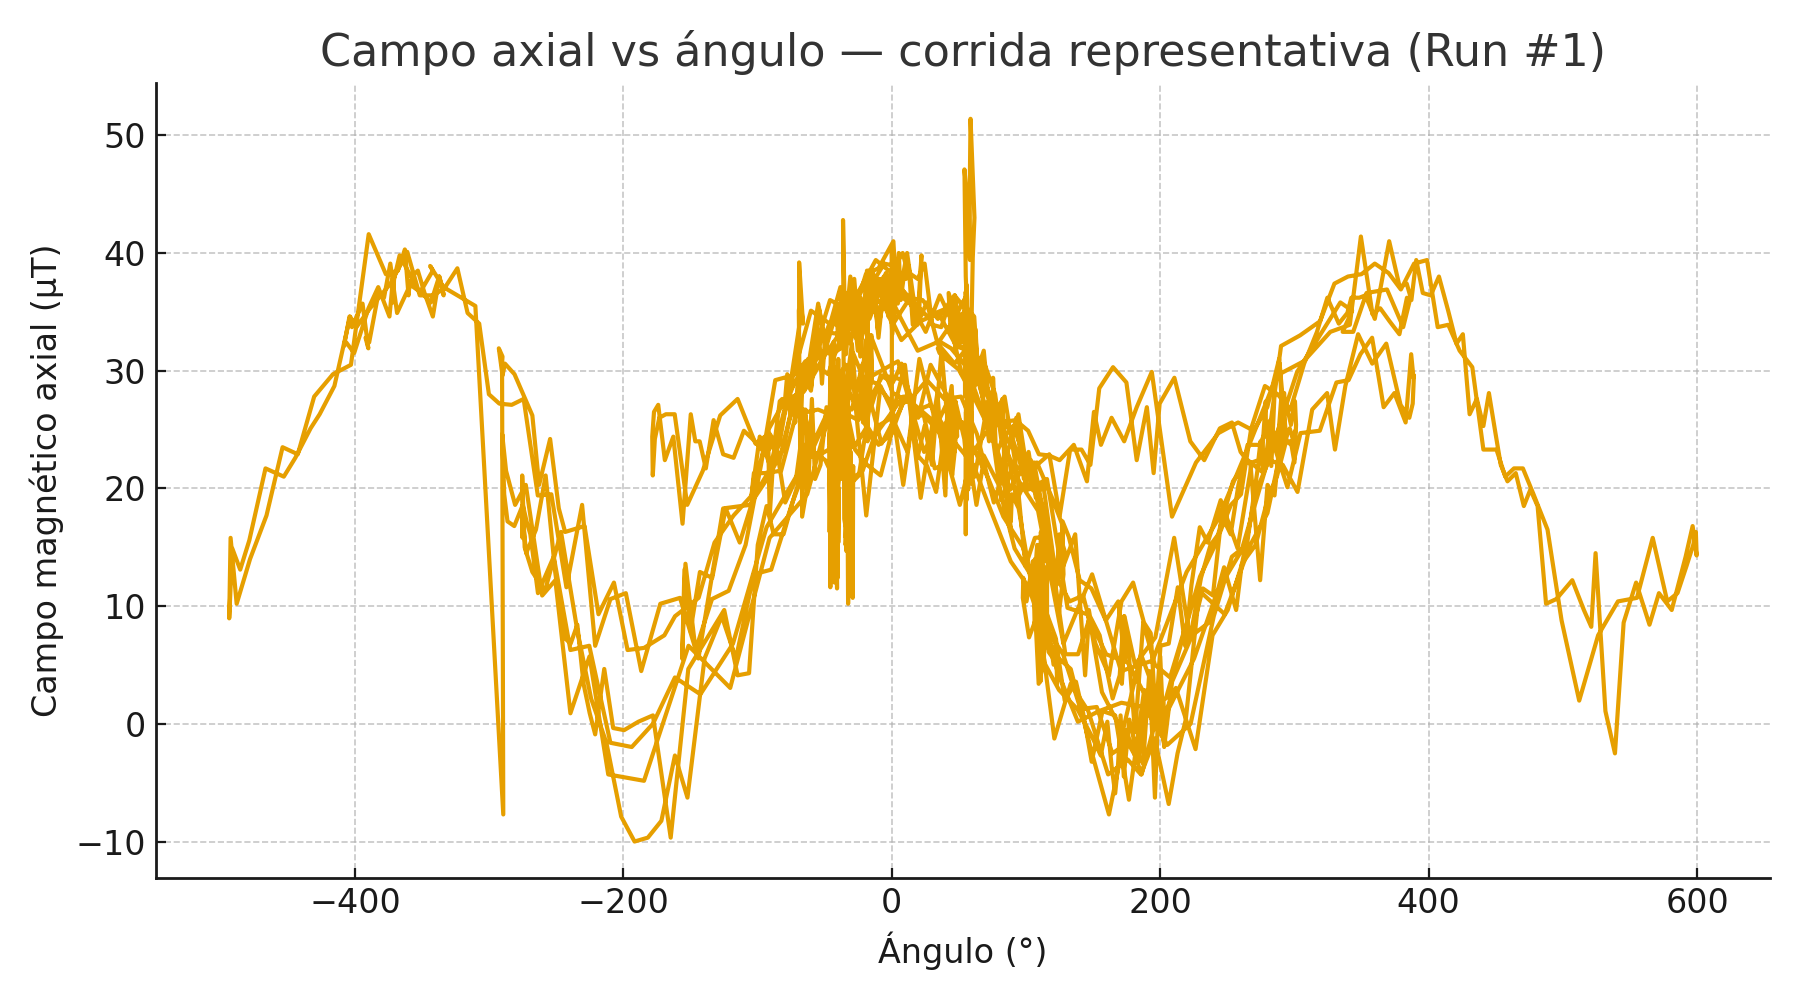
\includegraphics[width=0.8\textwidth]{figuras/grafico_horizontal.png}
    \caption{Ejemplo de curva sinusoidal obtenida en el plano horizontal. La amplitud corresponde a la componente \( B_\mathrm{H} \).}
    \label{fig:horizontal}
\end{figure}

\begin{figure}[H]
    \centering
    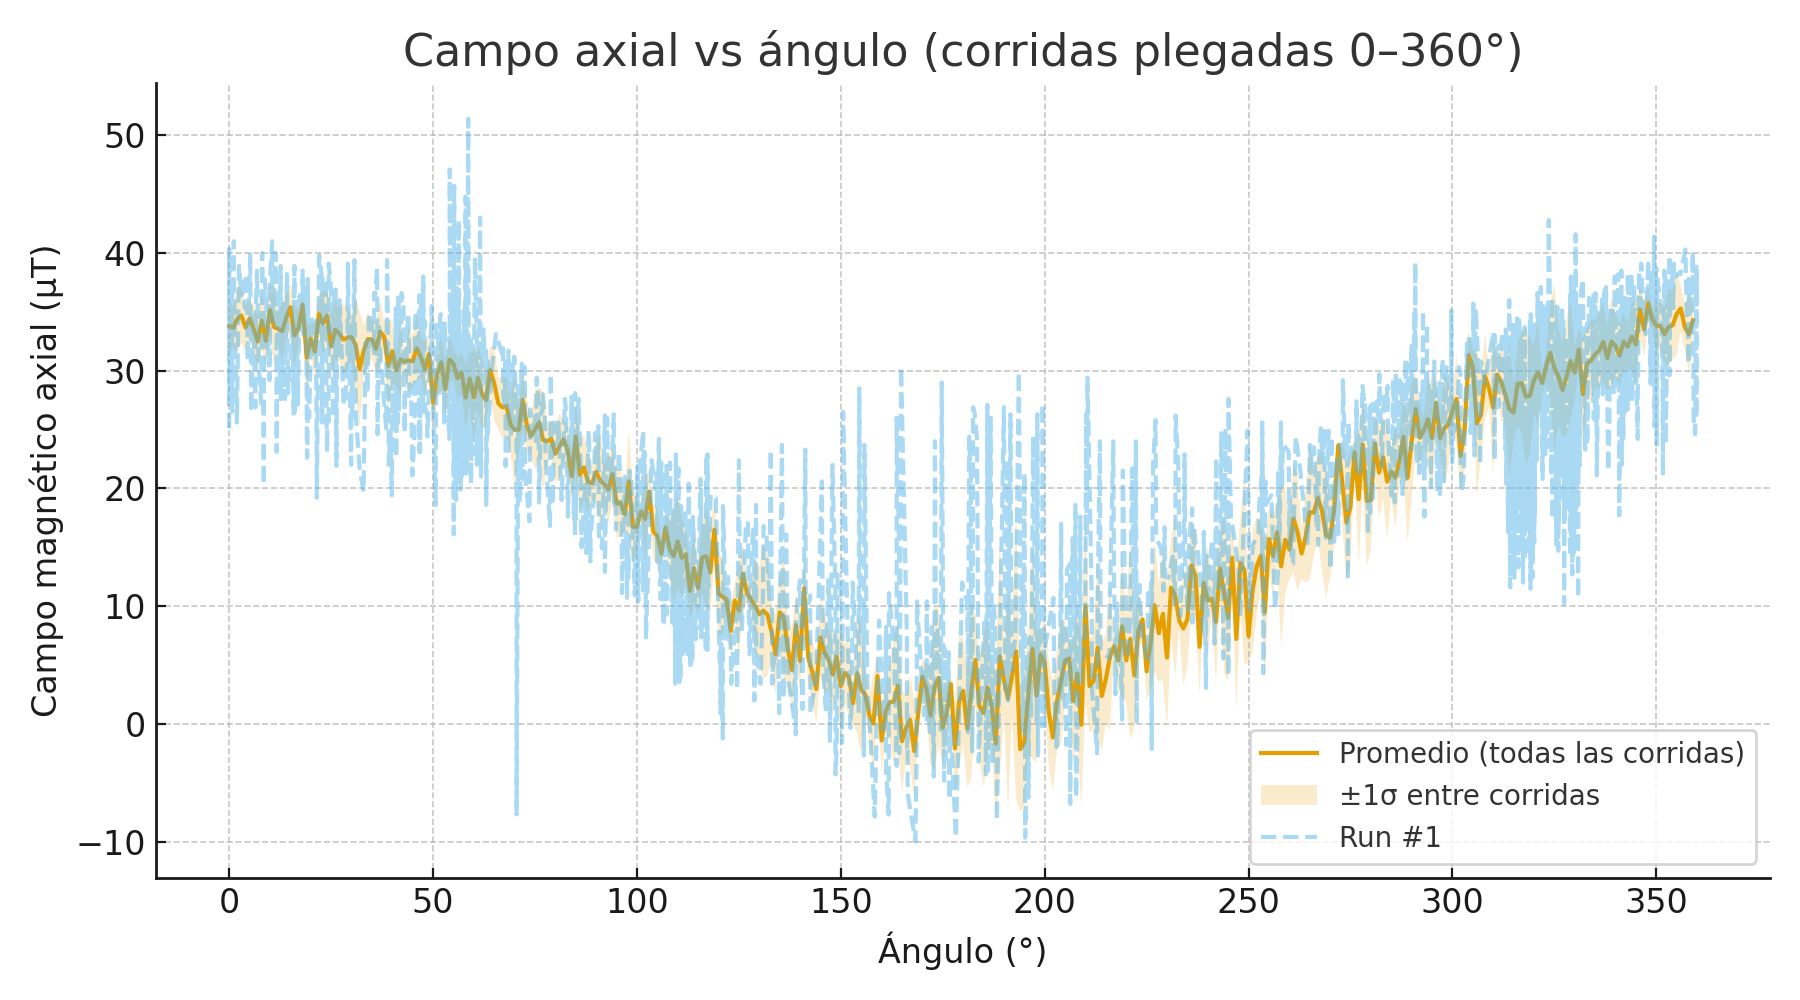
\includegraphics[width=0.8\textwidth]{figuras/grafico_vertical.png}
    \caption{Ejemplo de curva sinusoidal obtenida en el plano vertical. La amplitud corresponde a la componente \( B_\mathrm{T} \).}
    \label{fig:vertical}
\end{figure}

\vspace{1em}
La Figura~\ref{fig:horizontal} y la Figura~\ref{fig:vertical} muestran ejemplos representativos de las curvas sinusoidales utilizadas para extraer las amplitudes máximas. Estas curvas son típicas en este tipo de mediciones y presentan un comportamiento simétrico respecto al eje de rotación, con máximos en los ángulos correspondientes a la alineación con el campo terrestre.

\vspace{1em}
Como se aprecia en las figuras \ref{fig:horizontal} y \ref{fig:vertical}, la señal presenta un comportamiento claramente sinusoidal, con máximos bien definidos en la orientación alineada con el campo magnético terrestre. La dispersión observada en la Figura~\ref{fig:vertical} representa la variabilidad experimental entre corridas, que se mantuvo dentro de un margen controlado, reflejando una buena repetibilidad de la medición.

\vspace{1em}
Finalmente, la medición del ángulo de inclinación con la aguja de inmersión arrojó un valor de \(\theta_\text{aguja}\) cercano al valor calculado experimentalmente, reforzando la validez del procedimiento y del análisis realizado.



% ----------------- Discusión y Conclusiones -----------------
\section{Discusión y Conclusiones}

Los resultados experimentales obtenidos muestran una buena coherencia con el comportamiento esperado del campo magnético terrestre en la región. El valor promedio de la componente horizontal \( B_\mathrm{H} = 24.12 \pm 4.30~\si{\micro\tesla} \) y de la componente total \( B_\mathrm{T} = 34.40 \pm 2.47~\si{\micro\tesla} \) se encuentran próximos a los valores teóricos estimados para Uruguay, donde el modelo geomagnético WMM predice intensidades en el rango de \( 24{-}26~\si{\micro\tesla} \) para \( B_\mathrm{H} \) y alrededor de \( 36~\si{\micro\tesla} \) para \( B_\mathrm{T} \). El ángulo de inclinación obtenido experimentalmente (\( 45.5^\circ \)) es algo superior al valor de referencia (\( 37^\circ{-}40^\circ \)), pero la diferencia se encuentra dentro de un margen razonable considerando las limitaciones del montaje y las fuentes de error presentes.

Entre las principales fuentes de incertidumbre se destacan: (i) interferencias magnéticas locales producidas por estructuras metálicas cercanas o equipos eléctricos en funcionamiento, (ii) errores de alineación durante la rotación manual del sensor, y (iii) pequeñas variaciones en la calibración del sensor magnético y la cámara de cero gauss. Además, las condiciones experimentales no corresponden a un entorno de laboratorio completamente libre de perturbaciones externas, lo que contribuye a la dispersión observada en las mediciones, especialmente en \( B_\mathrm{H} \).

A pesar de estas limitaciones, la forma sinusoidal clara de las curvas y la buena concordancia de magnitudes demuestran la validez del método experimental empleado. El uso de un promedio de múltiples corridas permitió reducir el impacto del ruido y obtener un valor representativo del campo magnético terrestre local.

En conclusión, el procedimiento experimental permitió determinar de forma confiable la magnitud y dirección del campo magnético terrestre en el laboratorio. Los resultados obtenidos se encuentran en buen acuerdo con los valores teóricos esperados, evidenciando la validez del método basado en mediciones sinusoidales y el potencial de esta técnica para la enseñanza de conceptos de electromagnetismo en contextos experimentales reales.


% ----------------- Bibliografía -----------------
\begin{thebibliography}{9}

\bibitem{serway}
R.~A. Serway and J.~W. Jewett, \textit{Física para Ciencias e Ingeniería}, 9na ed., Cengage Learning, México, 2017.

\bibitem{pasco2}
PASCO Scientific, \textit{Práctico N°2: Campo Magnético de la Tierra}. Manual del sistema de laboratorio PASCO Capstone. UTEC, 2025.

\bibitem{geomag}
NOAA National Centers for Environmental Information, ``World Magnetic Model,'' disponible en: \url{https://www.ngdc.noaa.gov/geomag/} [Accedido: 20-oct-2025].

\bibitem{hyperphysics}
C.~R. Nave, ``Magnetic Field of the Earth,'' \textit{HyperPhysics}, Georgia State University. Disponible en: \url{http://hyperphysics.phy-astr.gsu.edu/hbase/magnetic/magearth.html} [Accedido: 20-oct-2025].

\bibitem{apa}
Normas APA. \url{http://www.cva.itesm.mx/biblioteca/pagina_con_formato_version_oct/apa.htm}

\end{thebibliography}

\end{document}
